\chapter{Vibrational Spectroscopies HREELS and IR}
Both the High Resolution Electron Energy Loss Spectroscopy (HREELS) and Infrared Adsorption Spectroscopy (IRAS) or just IR  rely on vibrational excitation of molecules adsorbed on surfaces. HREELS can in general only be used on nice and plane single crystal surfaces under UHV conditions, whereas the IR method is much more applicable and can be used both on well defined surfaces (reflection IR) and on real catalysts (transmission IR and Diffuse Reflectance IR). It can even be used at relatively high pressures, making it useful for investigating real catalysts {\it in situ}. One of the advantages of using HREELS is that it can even go to very low frequencies meaning that energy losses due to phonons etc. can be investigated. The resolution in the IR experiments are usually much better than HREELS, but when molecules are adsorbed on surfaces the relaxation time is short due to the coupling  to the surface eliminating some of this advantage. For more extensive treatment of these methods we will refer to \cite{Ibach,Ertl,Zangwill}.

\section{High Resolution Electron Energy Loss Spectroscopy}
\subsection{Experimental Set-up}
The HREELS experiments refers as the name says to high energy resolution since the energy loss spectroscopy also comes in a version where that is not the case. Earlier in Chapter \ref{ch:ea} we saw how electrons generated by an electron gun could be used to investigate the various energy losses mechanisms such as plasmon energy losses or losses by ionisation. However, energy losses to vibrations and phonons are very small and cannot be observed if the energy distribution of the electrons is not very narrow, say, below \SI{10}{m\electronvolt}. The way to achieve monochromatised electron beams is by using low primary energies and then use an energy analyser to select the appropriate energy. This is illustrated in \autoref{fig:hreelssetup}.

\begin{figure}[h!]
	\begin{center}
	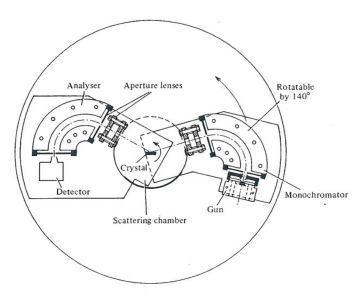
\includegraphics[scale=4]{figures/08_01.png}
	\caption{Schematics of a HREELS experiment.}
	\label{fig:hreelssetup}
	\end{center}
\end{figure}

The electrons are generated the usual way by heating a filament at a desired potential, the primary energy, which typically is less than \SI{10}{\electronvolt}. The electrons are then energy analysed by passing through an analyser, typically with a resolution in the range \SIrange{1}{5}{m\electronvolt}, and then  directed onto the sample. The electrons are interacting (reflected) with the sample and will in some cases also undergo an energy loss. The energy distribution of the reflected electrons is analysed by a second analyser which can be rotated around the specular direction. The experiment is not as easy to perform as those mentioned earlier. It is not trivial to get optimum resolution and at the same time a reasonable intensity. Also special precautions must be taken so that the slow electrons does not get detracted by any external fields, i.e. the set-up must be screened from magnetic fields (also the earth's field) by being incapsulated in a $\mu$-metal. The $\mu$-metal is a special alloy which leads the magnetic field lines in the metal screening the interior. Similarly the electron beam is also disturbed easily by changes in work function of the materials used in the analysers. The inside of the analyser is therefore coated with a graphite  ensuring a uniform work function.

\subsection{The Energy Loss Spectrum}
A typical HREEL spectrum is shown in \autoref{fig:cohreels}. At zero energy loss we find the elastically scattered electrons that have only been reflected from the surface. The overall resolution of the experiment is determined  by the FWHM of this elastic peak. The intensity of the energy losses are typically two orders of magnitude weaker and depends on the  nature of the excitation mechanism which can be  divided into dipole scattering and impact scattering.

\begin{figure}[h!]
	\begin{center}
	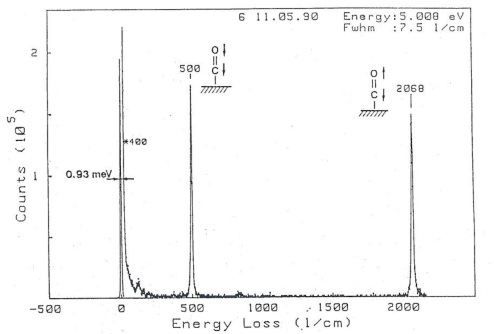
\includegraphics[scale=4]{figures/08_02.png}
	\caption{A HREEL spectrum of CO adsorbed on Ir(100). Notice that the resolution is below one \si{m\electronvolt}. Taken from \cite{Bruckmann}.}
	\label{fig:cohreels}
	\end{center}
\end{figure}

\subsubsection{Dipole Scattering}
In this mechanism the electron is first of all reflected elastically by the surface leading to a high intensity of electrons in the specular direction. An electron approaching a metal surface will set up a time dependent electric field that will be screened by the metal surface so that there is no field in the metal. This is described by an image charge with opposite sign travelling in the metal. The resulting electric field will be orthogonal to the surface and can be described in the frequency domain as

\begin{equation}
E(t)=\int E(\omega)e^{-i\omega t}d\omega
\end{equation}

This electric field will thus contain a frequency component equal to that of the vibrating molecule and couple with any dynamic (time-dependent) dipole moment on the surface. Consider for example a CO molecule adsorbed standing on the surface. The  CO molecule is polarised and possesses a very strong dynamic  dipole moment along the molecular axis. This dipole moment is further enhanced by the fact that the field from this dipole is screened by the metal resulting in a mirror dipole with the same sign. The interaction Hamiltonian for this will naturally be

\begin{equation}
{\bf H}_{int}\propto \vec{E}\cdot\vec{\mu}
\end{equation}
 
\noindent where $\vec{E}$ is the time-dependent electric field from the electron and $\vec{\mu}$ is the dipole moment operator for the CO molecule. The probability of exciting the vibration of the molecule will then again be given by Fermi's golden rule where

\begin{equation}
P_{if}=\vert <\Psi_i\vert{\bf H}_{int}\vert\Psi_f>\vert^2
\end{equation}

Since the electron undergoing the elastic scattering on the surface is setting up the electric field over a long range this energy loss may already start to happen when the electron is far from the surface ($<\SI{100}{\angstrom}$). The inelastic scattering is predominantly a forward scattering so the change in momentum to reflect the electron is supplied by the substrate.

It is now obvious that there will be a simple selection rule for the dipole scattering since vibrations involving dipoles parallel with the surface will be extinguished due to the metallic screening and no transitions will be possible. This is illustrated schematically in \autoref{fig:dipole}

It is seen that the probability depends strongly on the size of the dipole. For example CO has a strong dipole orthogonal to the surface when it is adsorbed in an up right position. This makes it possible to measure  even remote amounts of CO (typically a few per mille of a monolayer) on a surface. Unfortunately the size of the dipole is only constant in the low coverage regime. When the coverage increase the dipoles will start to interact with each other leading to screening and depolarisation so the energy loss intensity is no longer simply  proportional to the coverage. 

\begin{figure}[h!]
	\begin{center}
	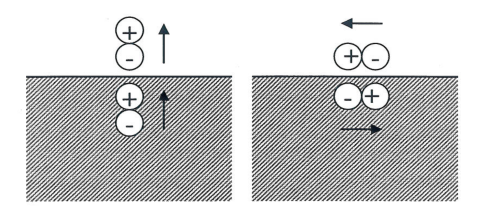
\includegraphics[scale=3]{figures/08_03.png}
	\caption{Sketch of the selection rules for dipole scattering.}
	\label{fig:dipole}
	\end{center}
\end{figure}

\subsubsection{Impact Scattering}
In the case of impact scattering  short range interactions are involved taking  place when the electron interact with the potential of the atoms i.e. distances  on the order of \SI{1}{\angstrom}. In this case the electrons are scattered over a wide range of angles and are, contrary to dipole scattering, not directed in the specular direction. The mechanism for excitations are also very different and there are no simple selection rules like in the dipole scattering. This means that in principle, it is possible to measure the dipole forbidden energy losses. Unfortunately the impact scattering is in general rather weak and is most often only observed when going away from the specular direction. Here the dipole component dies off rather quickly whereas the impact scattering persists as mentioned above as it is much more isotropic. In this manner it is possible to distinguish the two contributions from each other. It should for completeness' sake also be mentioned that there is a third mechanism called \emph{Negative ion resonances}. Here the electron is captured in an orbital forming a short lived negative intermediate losing energy before being re-emitted. 

\subsection{Experimental Results}
The method can be used to identify unknown intermediates on a surface and in some cases also be used to investigate the orientation of the adsorbate and even at what sort of site it is adsorbed. For example HREELS was used to identify that formate is formed when a Cu(100) crystal is exposed to several bars of \ce{CO2} and \ce{H2} at a temperature below \SI{363}{K}. The spectrum shows the energy losses characteristic for formate bound bidentate to the surface and the appropriate isotope shift for the C-H and C-D vibration was also found. The spectrum is shown in \autoref{fig:cuhreels}. Please note that it is also possible for the electrons to gain energy from excited vibrations if the population is sufficiently high.

\begin{figure}[h!]
	\begin{center}
	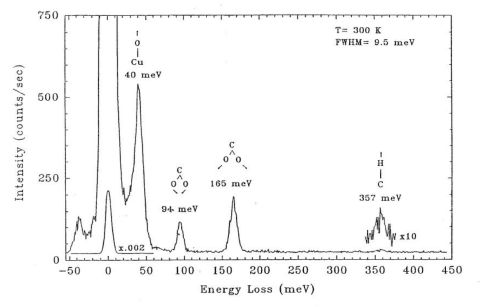
\includegraphics[scale=4]{figures/08_04.png}
	\caption{The HREEL spectra of the intermediates formed by exposing a Cu(100) crystal to gas mixtures of  \ce{CO2 + H2} and  \ce{CO2 + D2} respectively. The energy losses are characteristic for formate and the C-H vibration undergoes the expected shift upon isotropic labelling. Taken from \cite{Formate}}
	\label{fig:cuhreels}
	\end{center}
\end{figure}

Any gas phase molecule with $N$ atoms  will have $3N$ degrees of freedom. Thus a CO molecule in the gas phase will have 6 degrees of freedom, 3 translational, two rotational, and one vibrational mode. When the molecule adsorbs on the surface the rotational and translational modes become converted into frustrated vibrational modes as 2 frustrated rotational modes and 3 frustrated translational modes. Of these modes only the frustrated translational mode is orthogonal to the surface, dipole active, whereas the other modes usually only have weak dipoles in the surface plane and therefore forbidden. The different modes for atomic hydrogen and CO adsorbed on a substrate is shown in \autoref{fig:hcomodes}.

\begin{figure}[h!]
	\begin{center}
	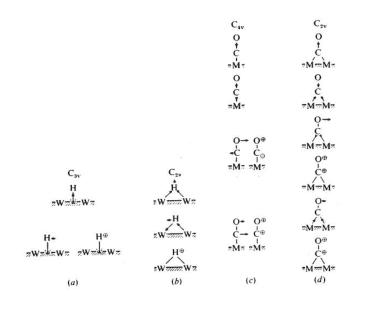
\includegraphics[scale=4]{figures/08_05.png}
	\caption{The number of modes of atomic hydrogen and CO in different adsorption symmetries. Degenerate mode are shown next to each other \cite{Bradshaw}.}
	\label{fig:hcomodes}
	\end{center}
\end{figure}

Thus only two energy losses should be expected for a CO molecule adsorbed standing up on the surface. These are observed at roughly \SI{260}{m\electronvolt} (C-O vibration) and at \SI{60}{m\electronvolt} (substrate-CO or frustrated translational mode, see Fig. \ref{fig:cohreels}). (Simply divide by 8 for conversion from \si{cm^{-1}} to \si{m\electronvolt}). The other modes should in principle also be observable in the off-specular mode where impact scattering dominate, but they are weak and have low frequencies making them difficult to observe on the high background from the elastic peak. One example where the number of the dipole forbidden modes have been used to identify the bonding site is H on W \cite{Barnes} (see Fig. \ref{fig:hwhreels}). Here the vibration of the H atom normal to the surface is easily identified in specular scattering as  $\nu_1$. However when going away from the specular direction two other modes are  identified as the two translational frustrated modes along the surface. Since there are two and not one mode, which then would be degenerated, the H atom must be bridge bonded since an on top or a  four fold hollow site would lead to degeneration of $\nu_2$ and $\nu_3$.

\begin{figure}[h!]
	\begin{center}
	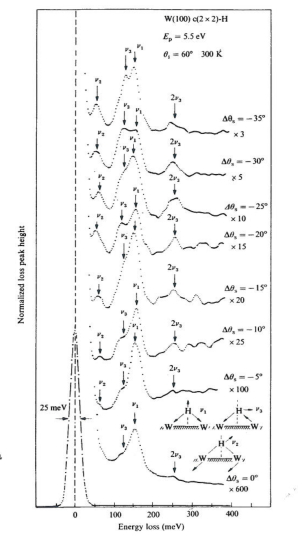
\includegraphics[scale=4.2]{figures/08_06.png}
	\caption{HREEL spectra of H-W(100)$(\sqrt{2}x\sqrt{2})$R\ang{45} measured with an electron beam with primary energy of \SI{5.5}{\electronvolt} at \ang{60} \cite{Barnes}.}
	\label{fig:hwhreels}
	\end{center}
\end{figure}

The size of the energy loss for a specific surface mode may also give information on the bonding site, although much care must be exercised here. According to Effective Medium Theory (EMT) any adsorbate will adsorb on a surface in a distance from the surface where it obtains its optimum electron density $n_s$. The binding energy will always have a minimum as a function of $n_s$ since at low electron density there are no overlap and thus no binding and at the very high electron density the Pauli repulsion takes over. Thus in this simple picture the bonding geometry only depends on $n_s$ and there will be no distinction between different adsorption sites like on-top, bridge or hollow sites. There are, however corrections to this model where the binding energy is  given by  

\begin{equation}
\Delta_{Bonding}=E(n_s)+E_{AS}+E_{1El}
\end{equation}

These correction terms determines where the adsorption will take place. The term $E_{AS}$, which is the Atomic Sphere correction, describes the repulsion occurring when to atoms comes close to each other. This means that it is in general most favourable for atoms to adsorb in high coordination sites since this gives the highest distance to the other atoms  minimising the repulsion term when located in the optimum electron density. This explains why species like carbon, nitrogen, oxygen and sulphur usually are found in three or four fold hollow sites. When this is not the case it is due to the last  correction term, the one electron correction.

\begin{figure}[h!]
	\begin{center}
	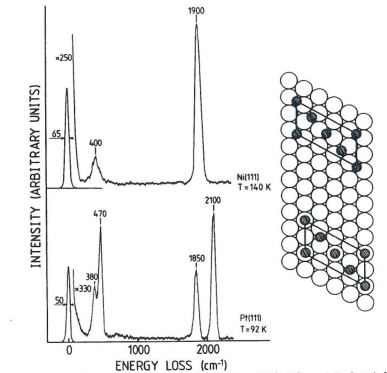
\includegraphics[scale=4]{figures/08_07.png}
	\caption{HREEL spectra of CO adsorbed on Ni(111) and Pt(111) \cite{Ibach}.}
	\label{fig:conipthreels}
	\end{center}
\end{figure}

Which trends can then be expected for atoms adsorbed on different sites on the surface? It is obvious that an atom sitting in a fourfold coordinated site will feel a much slower variation in the electron density (and thus the resulting binding potential) as it vibrates orthogonal to the surface compared to an atom sitting for example in an  on top site. In the  latter case there will in principle  only be  one atom to supply the necessary electron density and as the electron density decays exponentially from the atom in the EMT the potential will vary much faster resulting in a steeper potential and thus in a higher frequency.  Thus the trends for vibration energies  predicted from this simple picture are hollow < bridge < on top adsorption sites.
An example of this behavior is shown in \autoref{fig:conipthreels} where the HREEL spectra of CO adsorbed on Ni(111) and Pt(111) are shown.  It is seen how the on top sites on Pt(111) leads to a significantly higher frequency for both the energy losses to CO.

\section{Infrared Adsorption Spectroscopy}
Infrared spectroscopy is well known from analysis of chemical compounds in the gas phase. It can also be used for studying adsorbates on solid surfaces. One way to this is very similar to the HREELS experiment where the infrared light is deflected from a plane surface for example a single crystal surface.  This method is referred to as Infrared Reflectance Adsorption Spectroscopy (IRAS) or (RAIRS) depending on where the "infrared" is put in. Here the light is send in nearly parallel to the surface and again only the components that are dipole active on the surface may adsorb the light. The reflected light is measured and the absorbance can be measured. The advantage here is that it is possible to measure in a background of gas although care should be taken not to confuse gas phase adsorption  with adsorbate adsorbtion. 

The greatest advantage of IR is that it can be used to study real catalysts {\it in situ} in the transmission or reflectance mode. In the first case less than \SI{0.1}{g} of catalyst is  pressed into a thin disk a few tenths of a \si{mm} thick. Transmission IR can then be used if the absorbance of the catalyst support material is low. This is typically the case when using oxides and considering wavenumbers greater than \SI{1000}{cm^{-1}} which is equivalent to \SI{125}{m\electronvolt}. It is also important that the size of the catalyst particles are smaller than the wavelength of the infrared light since otherwise scattering would ruin the experiment. Often the absorbance of the catalyst itself make transmission impossible and then Diffuse Reflectance Infrared  Fourier Transform Spectroscopy (DRIFTS) may be used to measure the adsorbtion by surface species. Here the diffuse light scattered from a powder sample of catalyst is collected and analysed. Just as in the transmission mode the adsorbtion is measured and it is in this manner possible to study different intermediates adsorbed on the catalyst while running in almost realistic conditions taking the same precautions as mentioned above. By comparing observed absorbance bands to those measured on well defined surfaces it is possible to identify various species on the active catalyst. An important step towards closing the material gap. \autoref{fig:driftspec} depicts a typical DRIFT spectrum of  methanol synthesis.

\begin{figure}[h!]
	\begin{center}
	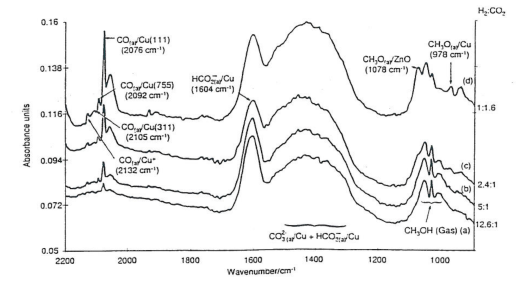
\includegraphics[scale=4]{figures/08_08.png}
	\caption{DRIFT spectrum of a working methanol catalyst \ce{Cu / ZnO / Al2O3} in steady state at \SI{30}{bar} and \SI{413}{K} taken from \cite{Bailey}.}
	\label{fig:driftspec}
	\end{center}
\end{figure}